\documentclass[journal,12pt,twocolumn]{IEEEtran}

\usepackage{graphicx}
\usepackage{setspace}
\usepackage{gensymb}
\singlespacing
\usepackage[cmex10]{amsmath}
\usepackage{amssymb}
\usepackage{xurl}
\usepackage{tabularx}
\usepackage{amsthm}
\usepackage{comment}
\usepackage{mathrsfs}
\usepackage{txfonts}
\usepackage{stfloats}
\usepackage{bm}
\usepackage{cite}
\usepackage{cases}
\usepackage{subfig}
\usepackage{arydshln}
\usepackage{longtable}
\usepackage{multirow}

\usepackage{enumitem}
\usepackage{mathtools}
\usepackage{steinmetz}
\usepackage{tikz}
\usepackage{circuitikz}
\usepackage{verbatim}
\usepackage{tfrupee}
\usepackage[breaklinks=true]{hyperref}
\usepackage{graphicx}
\usepackage{tkz-euclide}
\usetikzlibrary{automata, positioning}
\usetikzlibrary{calc,math}
\usepackage{listings}
    \usepackage{color}                                            %%
    \usepackage{array}                                            %%
    \usepackage{longtable}                                        %%
    \usepackage{calc}                                             %%
    \usepackage{multirow}                                         %%
    \usepackage{hhline}                                           %%
    \usepackage{ifthen}                                           %%
    \usepackage{lscape}     
\usepackage{multicol}
\usepackage{chngcntr}
\usepackage{blkarray}

\DeclareMathOperator*{\Res}{Res}

\renewcommand\thesection{\arabic{section}}
\renewcommand\thesubsection{\thesection.\arabic{subsection}}
\renewcommand\thesubsubsection{\thesubsection.\arabic{subsubsection}}

\renewcommand\thesectiondis{\arabic{section}}
\renewcommand\thesubsectiondis{\thesectiondis.\arabic{subsection}}
\renewcommand\thesubsubsectiondis{\thesubsectiondis.\arabic{subsubsection}}


\hyphenation{op-tical net-works semi-conduc-tor}
\def\inputGnumericTable{}                                 %%

\lstset{
%language=C,
frame=single, 
breaklines=true,
columns=fullflexible
}
\begin{document}


\newtheorem{theorem}{Theorem}[section]
\newtheorem{problem}{Problem}
\newtheorem{proposition}{Proposition}[section]
\newtheorem{lemma}{Lemma}[section]
\newtheorem{corollary}[theorem]{Corollary}
\newtheorem{example}{Example}[section]
\newtheorem{definition}[problem]{Definition}

\newcommand{\BEQA}{\begin{eqnarray}}
\newcommand{\EEQA}{\end{eqnarray}}
\newcommand{\define}{\stackrel{\triangle}{=}}
\bibliographystyle{IEEEtran}
\raggedbottom
\setlength{\parindent}{0pt}
\providecommand{\mbf}{\mathbf}
\providecommand{\pr}[1]{\ensuremath{\Pr\left(#1\right)}}
\providecommand{\qfunc}[1]{\ensuremath{Q\left(#1\right)}}
\providecommand{\sbrak}[1]{\ensuremath{{}\left[#1\right]}}
\providecommand{\lsbrak}[1]{\ensuremath{{}\left[#1\right.}}
\providecommand{\rsbrak}[1]{\ensuremath{{}\left.#1\right]}}
\providecommand{\brak}[1]{\ensuremath{\left(#1\right)}}
\providecommand{\lbrak}[1]{\ensuremath{\left(#1\right.}}
\providecommand{\rbrak}[1]{\ensuremath{\left.#1\right)}}
\providecommand{\cbrak}[1]{\ensuremath{\left\{#1\right\}}}
\providecommand{\lcbrak}[1]{\ensuremath{\left\{#1\right.}}
\providecommand{\rcbrak}[1]{\ensuremath{\left.#1\right\}}}
\theoremstyle{remark}
\newtheorem{rem}{Remark}
\newcommand{\sgn}{\mathop{\mathrm{sgn}}}
\providecommand{\abs}[1]{\vert#1\vert}
\providecommand{\res}[1]{\Res\displaylimits_{#1}} 
\providecommand{\norm}[1]{\lVert#1\rVert}
%\providecommand{\norm}[1]{\lVert#1\rVert}
\providecommand{\mtx}[1]{\mathbf{#1}}
\providecommand{\mean}[1]{E[ #1 ]}
\providecommand{\fourier}{\overset{\mathcal{F}}{ \rightleftharpoons}}
%\providecommand{\hilbert}{\overset{\mathcal{H}}{ \rightleftharpoons}}
\providecommand{\laplace}{\overset{\mathcal{L}}{ \longleftrightarrow}}
	%\newcommand{\solution}[2]{\textbf{Solution:}{#1}}
\newcommand{\solution}{\noindent \textbf{Solution: }}
\newcommand{\cosec}{\,\text{cosec}\,}
\providecommand{\dec}[2]{\ensuremath{\overset{#1}{\underset{#2}{\gtrless}}}}
\newcommand{\myvec}[1]{\ensuremath{\begin{pmatrix}#1\end{pmatrix}}}
\newcommand{\mydet}[1]{\ensuremath{\begin{vmatrix}#1\end{vmatrix}}}
\newcommand*{\permcomb}[4][0mu]{{{}^{#3}\mkern#1#2_{#4}}}
\newcommand*{\perm}[1][-3mu]{\permcomb[#1]{P}}
\newcommand*{\comb}[1][-1mu]{\permcomb[#1]{C}}
\numberwithin{equation}{subsection}
\makeatletter
\@addtoreset{figure}{problem}
\makeatother
\let\StandardTheFigure\thefigure
\let\vec\mathbf
\renewcommand{\thefigure}{\theproblem}
\def\putbox#1#2#3{\makebox[0in][l]{\makebox[#1][l]{}\raisebox{\baselineskip}[0in][0in]{\raisebox{#2}[0in][0in]{#3}}}}
     \def\rightbox#1{\makebox[0in][r]{#1}}
     \def\centbox#1{\makebox[0in]{#1}}
     \def\topbox#1{\raisebox{-\baselineskip}[0in][0in]{#1}}
     \def\midbox#1{\raisebox{-0.5\baselineskip}[0in][0in]{#1}}
\vspace{3cm}
\title{\textbf{ GATE ASSIGNMENT 3}}
\author{Dhatri Nanda - AI20BTECH11002}
\maketitle
\newpage
\bigskip
\renewcommand{\thefigure}{\arabic{figure}}
\renewcommand{\thetable}{\arabic{table}}
Download all python codes from 
\begin{lstlisting}
https://github.com/Dhatri-nanda/EE3900/blob/main/Gate_3/code.py
\end{lstlisting}
%
Download latex-tikz codes from 
%
\begin{lstlisting}
https://github.com/Dhatri-nanda/EE3900/blob/main/Gate_3/Gate_3.tex
\end{lstlisting}
\section*{QUESTION}
The impulse response functions of four linear systems $S_1,S_2,S_3,S_4$ are given respectively by 
\begin{align}
    h_1(t) &= 1\\
    h_2(t) &= U(t)\\
    h_3(t) &= \frac{U(t)}{t+1}\\
    h_4(t) &= e^{-3t}U(t)
\end{align}
where $U(t)$ is the unit step function, which of these systems is time invariant, casual and stable?
\begin{enumerate}[label={\alph*)}]
\begin{multicols}{4}
\setlength\itemsep{2em}
\item $S_1$\\
\item $S_2$\\
\item $S_3$\\
\item $S_4$\\
\end{multicols}
\end{enumerate}
\section*{SOLUTION}
Definitions:-
\begin{enumerate}
    \item A continuous time signal x(t) is said to be \textbf{casual} if $x(t) = 0$ for every $t<0$.\\
    \item A time dependant system that is not a direct function of time is called \textbf{time-invariant} system.\\
    \item A continuous time system is \textbf{stable} if and only if all the poles of it's transfer function occur in the left half of the complex plane. Whereas marginal stability correlates with zero real part.\\
    \item A continuous time system $h(t)$ is said to be BIBO stable if and only if it is absolutely integrable
    \begin{align}
        \int_{-\infty}^{\infty} h(t)dt < \infty
    \end{align}
\end{enumerate}
    The transfer function of an impulse response function by using laplace transform is
    \begin{align}
    H(s) = \mathcal{L}\cbrak{h(t)}(s) = \int_{-\infty}^{\infty} h(t)e^{-st} dt
    \end{align}
    U(t) is given as the unit step function,
\begin{align}
    U(t) = 
    \begin{cases}
    0, t<0\\
    1, t\geq 0
    \end{cases} \label{eq 0.0.6}
\end{align}
Given, {$h_1(t) = 1$}

It is a non casual system as $h_1(t) \neq 0$ for any $t<0$\\
And, since it is not a time dependant function, it is not time-invariant.\\
Next, the transfer function of $h_1(t)$ is
\begin{align}
    H_1(s) &= \int_{-\infty}^{\infty} e^{-st} dt\\
    &= \sbrak{\frac{e^{-st}}{s}}_{-\infty}^{\infty} = \infty
\end{align}
The transfer function is not defined, so we cannot decide the stability. 

$\therefore$ We check the BIBO stability.

\begin{align}
    &= \int_{-\infty}^{\infty} U(t) dt\\
    &= \int_0^{\infty} 1 dt\\
    &= \sbrak{t}_0^{\infty} = \infty
\end{align}
$\therefore$ The system $S_1$ is not stable.\\\\
Given, $h_2(t) = U(t)$

From \eqref{eq 0.0.6}
\begin{align}
    h_2(t) = 
    \begin{cases}
    0, t<0\\
    1, t\geq 0
    \end{cases}
\end{align}

It satisfies the condition for casuality.So, system $S_2$ is casual.

It is also time-invariant by the above given definition.

The transfer function of $h_2(t)$ is
    \begin{align}
        H_2(t) &= \int_{-\infty}^{\infty} U(t)e^{-st} dt\\
        &= \int_{0}^{\infty} e^{-st} dt\\
        &= \frac{1}{s}
    \end{align}
Pole is $s = 0$ and ROC is $ \mathcal{R}e\cbrak{s} > 0$

$\therefore$ The system $S_2$ is marginally stable.
\begin{figure}[htp]
    \centering
    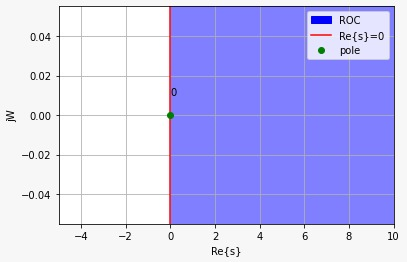
\includegraphics[width=\columnwidth]{onee.png}
    \caption{plot for $H_2(t)$}
    \label{fig:my_label}
\end{figure}\\\\\

Given, $h_3(t) = {U(t)}/{(t+1)}$

From, \eqref{eq 0.0.6}
\begin{align}
    h_3(t) = 
    \begin{cases}
    0, {t<0, t \neq -1}\\
    \text{not defined}, t = -1\\
    \frac{1}{t+1} , t > 0
    \end{cases}
\end{align}

The system is not casual because 
\begin{align}
h_3(t) \neq 0, t = -1
\end{align}
The denominator of $h_3(t)$ is a direct function of time, so it is not time-invariant.

The transfer function of $h_3(t)$ is
\begin{align}
    H_3(t) &= \int_{-\infty}^{\infty} \frac{U(t)}{t+1}e^{-st} dt\\
    &= \int_{0}^{\infty} \frac{e^{-st}}{t+1} dt
\end{align}
Substituting x = st + s 
$\implies \frac{dx}{dt} = s$ $\implies dt = \frac{1}{s}dx$
\begin{align}
    &= \int_{s}^{\infty} \frac{e^x}{x} dx
\end{align}
The above integral is not a definite integral. \\
So, 
\begin{align}
    H_3(t) = \infty
\end{align}
As the transfer function is not defined, we check the BIBO stability.

\begin{align}
   &= \int_{-\infty}^{\infty} \frac{U(t)}{t+1} dt\\
    &= \int_0^{\infty} \frac{1}{t+1} dt\\
    &= \sbrak{log(t+1)}_0^{\infty} = \infty
\end{align}
$\therefore$ The system $S_3$ is not stable.\\

Given, $h_4(t) = e^{-3t}U(t)$

From \eqref{eq 0.0.6}
\begin{align}
    h_4(t) = 
    \begin{cases}
    0, t<0\\
    e^{-3t}, t\geq 0
    \end{cases}
\end{align}
It satisfies the condition for casuality. So the system is casual.

As $e^{-3t}$ is a direct function of time, the system is not time-invariant.

The transfer function of $h_4(t)$ is 
\begin{align}
    H_4(t) &= \int_{-\infty}^{\infty} e^{-3t}U(t)e^{-st} dt\\
    &= \int_{0}^{\infty} e^{-(3+s)t} dt\\
    &= \frac{1}{3+s}
\end{align}
Pole is $s = -3$ and ROC is $\mathcal{R}e\cbrak{s} > -3$

$\therefore$ $S_4$ is a stable system.

\begin{figure}[htp]
    \centering
    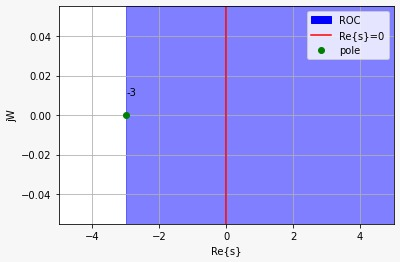
\includegraphics[width=\columnwidth]{twoo.png}
    \caption{plot for $H_4(t)$}
    \label{fig:my_label}
\end{figure}

\textbf{Our Results:}\\\\
\begin{tabular}{|p{2cm}||p{1.5cm}|p{1.5cm}|p{1.5cm}|}
     \hline
     System & casual & stable & time-invariant\\
     \hline
     1 & no & no & no\\
     \hline
     $U(t)$ & yes & yes & yes\\
     \hline
     $U(t)/(t+1)$ & no & no & no\\
     \hline
     $e^{-3t}U(t)$ & yes & yes & no\\
     \hline
\end{tabular}\\

$\therefore$ option B is correct.
\end{document} 
